\documentclass[10pt, conference, compsocconf]{IEEEtran}

\usepackage{cite}
\usepackage{float}
\usepackage{tabularx}
\usepackage{makecell}
\usepackage{multirow}
\usepackage{amsmath,amssymb,amsfonts}
\usepackage{algorithmic,algorithm}
\usepackage{graphicx}
\usepackage{textcomp}
\usepackage{xcolor}
\usepackage{listings}
\usepackage[T1]{fontenc}
\graphicspath{{./images/}}
\def\BibTeX{{\rm B\kern-.05em{\sc i\kern-.025em b}\kern-.08em
    T\kern-.1667em\lower.7ex\hbox{E}\kern-.125emX}}
\begin{document}

\title{A Fully Decentralized Infrastructure for Subscription-based IoT Data Trading}

\author{\IEEEauthorblockN{Ching-Hua (Vivian) Lin}
\IEEEauthorblockA{dept. of CSIE\\
National Cheng Kung University\\
Tainan City, Taiwan (R.O.C.)\\
p76074591@gs.ncku.edu.tw}
\and
\IEEEauthorblockN{Ching-Chun (Jim) Huang}
\IEEEauthorblockA{dept. of CSIE\\
National Cheng Kung University\\
Tainan City, Taiwan (R.O.C.)\\
jserv@ccns.ncku.edu.tw}
\and
\IEEEauthorblockN{Yang-Hao Yuan}
\IEEEauthorblockA{BiiLabs Co., Ltd.\\
Taiwan (R.O.C.)\\
yanghau@biilabs.io}
\and
\IEEEauthorblockN{Zih-shiuan (Spin) Yuan}
\IEEEauthorblockA{BiiLabs Co., Ltd.\\
Taiwan (R.O.C.)\\
spin@biilabs.io}
}


\maketitle


\begin{abstract}
On top of subscription-based pricing models such as Software-as-a-Service (SaaS), monetizing the subscription enables the payment of data streams with data usage instead of a particular price for a fixed data set. This pricing model allows data providers to have a better vision of managing budgets and data consumers to have the flexibility to subscribe and unsubscribe. However, unlike static data collections, the streaming data increases difficulties of dynamic data ownership and identity verification. A trustless data trading infrastructure is required where the entities can trade, validate data ownership and data integrity without trusting any service or participants. In addition, an automated subscription procedure is also demanded for the sake of data monetization. In this paper, we leverage usages of distributed ledger technologies (DLTs) to construct a decentralized data trading platform on top of the IoT brokered infrastructure. This approach can efficiently enhance the degree of transparency and scalability. The storage built upon cryptographic message protocols allows transmitting, accessing and validating data streams over distributed ledgers without authorities, and the digital rights of trading participants deserve a guarantee, which is enabled by design.
\end{abstract}

\begin{IEEEkeywords}
subscription model, decentralization, data monetization
\end{IEEEkeywords}

\section{Introduction}
As the physical and digital data are deeply intertwined in IoT, the interactions among digital twins act as data exchanges\cite{digitaltwin} which brings potential value to IoT applications, such as health care, factories, and vehicles, and brings up new business models where data is considered as tradeable digital assets. With the diverse data streams generated by different entities and carried across organizations among expanding the number of interconnected devices, it is a challenge for data holders to share and track their data assets. Therefore, the data trading platform is viewed as a solution to build a secure, reliable, and scalable data sharing mechanism where data providers and data consumers meet.

In contrast to the existing solutions targeting static data sets\cite{DIaas, MARSA}, this paper aims for processing the high volume, high velocity, and high variety of real-time data streams\cite{BigData}. As streaming data is composed of records at every moment, users or devices are interested in data of a specific time period instead of the whole timeline. For example, the Internet of Vehicles (IoV) allows vehicles to connect with traffic signs and bicycles, share information, and at the same time be able to understand the real-time environmental conditions and find the best route through the communication. While vehicles and traffic lights continuously generate information, a device only needs to process the data streams of surroundings but all appliances in the IoV.

In data trading platforms, there are three major aspects that need trust: identity, data ownership, and trading.
Among the challenges of data trading platform\cite{BigDataMarket}, the following characteristics are required:
\begin{itemize}
    \item \textbf{Scalability}.
1) The performance of the platform should scale with the massive amount of participants. 2) The keys and entry points of data products managed by participants should be as small as possible.
    \item \textbf{Integrity}. 1) Prevent unauthorized modifications. 2) Ensure the accuracy and validity of contents.
    \item \textbf{Confidentiality}.
1) Only the authorized participants can access data streams. 2) Participants that have access can always retrieve data even if they're dropped from the network.
    \item \textbf{Privacy}. Avoid revealing sensitive information of all participants, such as IP address and data consumers' habits which may leak within the subscription history.
\end{itemize}

Taking all the requirements into consideration, we investigate the use of decentralized publish/subscribe (pub/sub) model and DLTs to construct the authority-less and trusted infrastructure as shown in Fig.~\ref{fig:system_design}. The pub/sub model features the scalability and resource-efficiency, and DLTs resolve the trust of the service, since data and contracts written on DLTs are transparent, immutable, and enforced automatically, which allows devices to focus on their jobs while gaining the rewards. Lastly, an end-to-end encrypted transmission protocol built on top of DLT is used as data storage, which not only ensures the data integrity but also enables access control and provides a scalable key and data management.

\begin{figure}[!t]
    \centering
    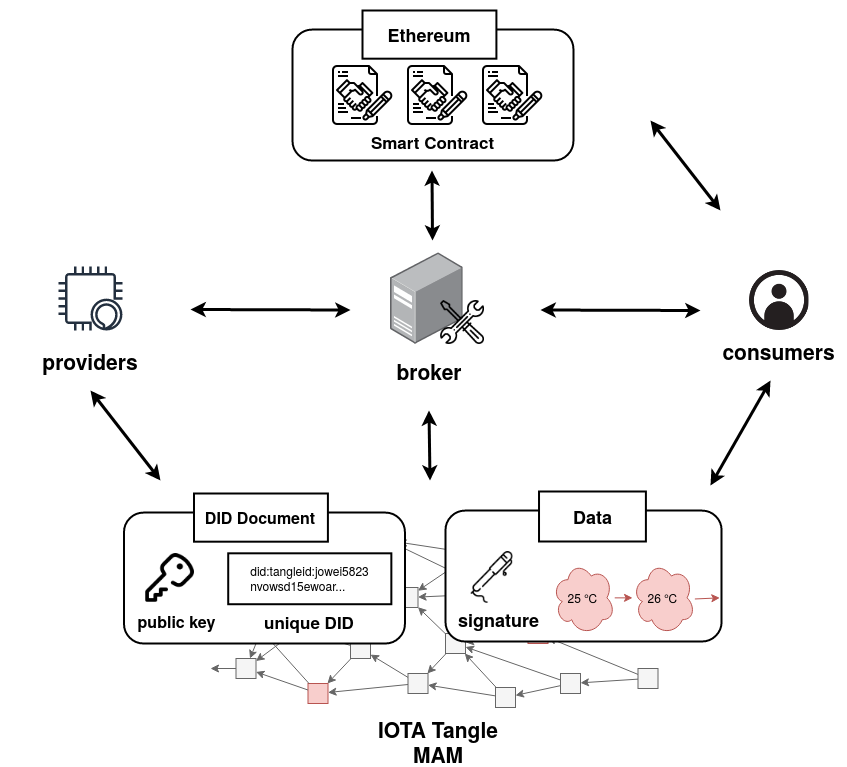
\includegraphics[width=3.in]{system_design}
    \caption{The system design of a decentralized data trading infrastructure which consists of data providers, consumers and brokers.}
    \label{fig:system_design}
\end{figure}

\section{Related Work}
\label{section:relatedWork}
G. S. Ramachandran et al.\cite{trinity} pointed out the security risk of centralized brokers, and applied DLTs to build a distributed pub/sub system which promotes the transparency of interactions of participants and the status of data. Data validation and traceability are achieved via the Ethereum smart contract. But data is plaintext on blockchain that the system is not appropriate for sensitive data.

Secure Pub-Sub model\cite{SPS}, a brokerless design, is proposed to eliminate the security risk of middleware and to provide a reputation-based fairness payment strategy on blockchain.
The privacy and data security are considered thoroughly with the encryption scheme, while the reputation of publishers, payment, and data sharing are deployed on smart contracts that allow all operations are transparent. Yet, without brokers, participants may need to reveal more sensitive information in order to communicate. By Paolo Missier et. al\cite{MindMyValue} presenting an IoT brokered infrastructure based marketplace which enables trading with Ethereum smart contracts. The brokers are only responsible for data transmission in order to adapt flexible agreement between participants. However, the data cubes (i.e., a tuple of data information) are stored in a centralized Cassandra database, guaranteed to be tamper-proof but the risk of single-point failure still exists.

Masked Authenticated Messaging (MAM)\cite{MAM} is regarded as a secure data transmission layer and data storage built on top of DLT which provides access control, tamper-proof, and authentication functionalities by tailoring messages to a channel. The industrial data marketplace\cite{IOTAIdustryMarketplace} proposed by IOTA Foundation targets for IoT data streams trading in IOTA token and applies MAM as the data storage and data transmission layer. The decentralized data marketplace\cite{DDMSmartCities} is operated without any intermediate server but data providers only, data providers attach, and trade data streams via MAM. Nevertheless, the above works did not take into account the refund and unsubscribe mechanism of the trading model.
 
\section{System Design Thinking}
\label{section:design_thinking}
\subsection{Data subscription-based trading platform players}
There are three major participants, data providers, data consumers and brokers in our proposed architecture.

\begin{itemize}
\item \textbf{Data Provider: }
Data providers are the ones that generate streaming data and set the data price based on the different types of data. With the subscription fee that earned via trading, data providers are incentivized to maintain and improve the quality of data.
\item \textbf{Data Consumer: }
Data consumers are entities that are willing to buy data streams. As it is laborious to widely deploy devices to collect data from scratch, and without a marketplace, it is also difficult to find providers of the data sets. Purchase is the fastest and efficient way to get the desired data sets.
\item \textbf{Broker: }
Brokers are responsible for building an agreement and handling trading processes between data providers and consumers. Brokers are required to be online for providers and consumers, and they are incentivized by charging brokerage fees.
\end{itemize}

Adopting brokers between providers and consumers has three advantages. First, considering the entities could be machines that are not online anytime, brokers can continue the trading process if either side is offline. Second, a fully decentralized architecture has difficulties to brings data providers and consumers together, both of them need to reveal more sensitive information, such as IP address, in order to build the communication tunnel. Brokers resolved the privacy issue, as brokers are the bridges that link data providers and consumers, participants can trade with minimum information like its identifier and public key. Third, a refund process needs brokers to host and supervise the procedures in order to protect the rights of participants, which will be further discussed in Section.~\ref{section:refund}.

\begin{figure}[h]
    \centering
    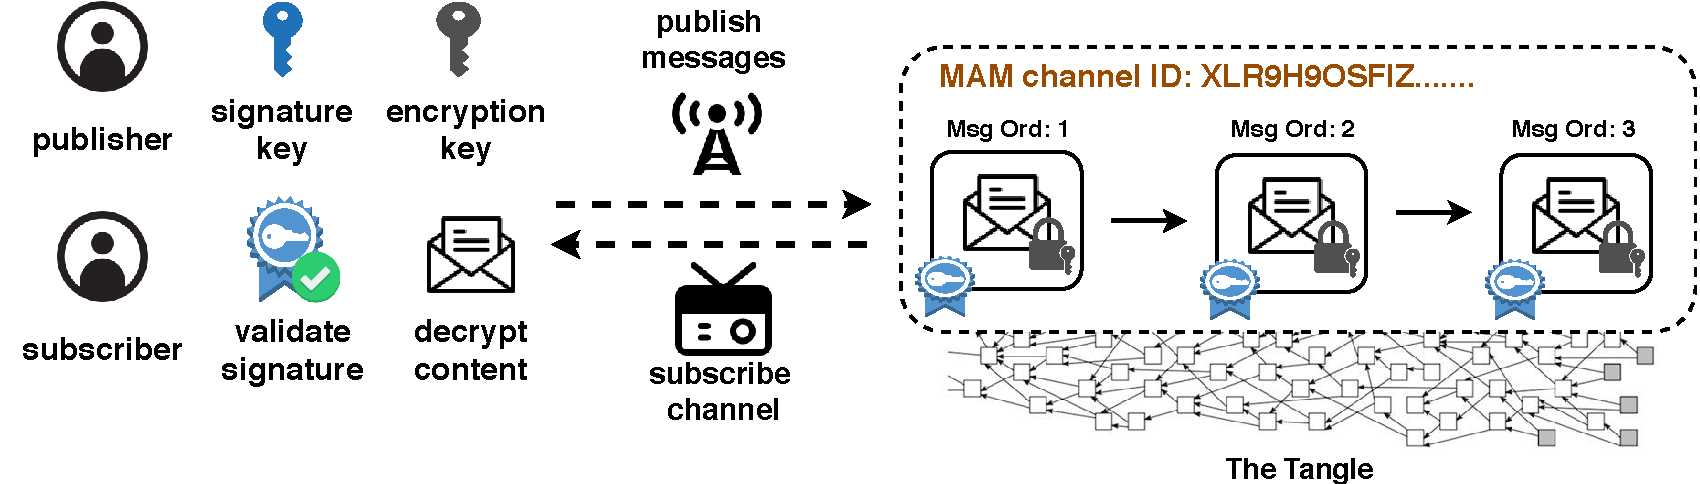
\includegraphics[width=3.5in]{channel_and_key_fold}
    \caption{Within MAM channel, the message publisher has 2 types of key, the encryption keys for content encryption and signature keys for digital signatures. Subscribers can validate the message with signature keys and decrypt messages with encryption keys.}
    \label{fig:channel_and_key}
\end{figure}

\subsection{Choice of Data Storage}
Data storage is the trust basis of data trading platforms where the data assets are reserved. Streaming data unlike a fixed set of data that can be verified by the hash of the whole pack of data consists of continually granular records of each time slot. Therefore, the verification such as data integrity and source identity is narrow down to a data point as well. In our proposed architecture, MAM is adopted as data storage to resolve the challenges of managing and verifying data streams by implementing the second layer data communication protocol built on top of the IOTA network, the Tangle, which has properties like publishing, classifying and tracking authenticated message streams. It builds the trust of the platform while meeting the requirements of IoT streaming data storage which can be concluded: 1) \textbf{Scalability}, for both data providers and consumers, MAM keeps the number of managed keys and data entry points as small as possible. 2) \textbf{Integrity}, messages were written on the Tangle are immutable. 3) \textbf{Confidentiality}, the message can be encrypted with an \textbf{encryption key} that restricts only authorized players can access contents. 4) \textbf{Proof of Ownership}, signing messages with \textbf{signature key} generated from Merkle signature scheme\cite{MSS} (MSS) allows users to ensure them originated from the same source by validating the signatures without knowing the actual contents. See Fig.~\ref{fig:channel_and_key} for illustration.

Using MAM as a data storage benefits from the underlying IOTA network as well as the decentralized and fault-tolerant characteristics, which reduce the risks of centralized storage services. Furthermore, the rights of data access are traded instead of a copy of data in the trading platform, which eliminates the need for data consumers to have additional storage.

However, the performance results of MAM operations, in Section.\ref{section:mam_performance} show that operating MAM requires lots of resources for the devices, therefore, we present an alternative solution for data providers to delegate these computing tasks to powerful proxy servers, Tangle-accelerator (Accel)\cite{TA}, while ensuring the privacy. The details would be further illustrated in Section.\ref{section:ta_endpoint}.

Currently, considering the efficiency of uploading large files, IPFS performs better than MAM (i.e., writing content to the IOTA network). However, IOTA network scales when more users and transactions join, and the MAM operations can be delegated. Furthermore, adopting IPFS in IoT scenarios may meet the challenges of data loss and data retrieving efficiency.

\subsection{Digital Identity}
The digital identity represents an entity and holds the digital assets within the digital world, it is important to prove and show the identity to others during interactions. We select the decentralized identity model rather than a centralized one for the concerns in Table.\ref{tab:did}.
\begin{table}[h]
    \caption{Identity models: centralized vs. decentralized}
    \label{tab:did}
    \begin{tabularx}{\linewidth}{|l|X|X|}
    \hline
        \textbf{Identity Model} & \textbf{Centralized} & \textbf{Decentralized} \\
        \hline
        Control & Enterprises control identities & Entities control their identities \\
        \hline
        Security & Identity held in a centralized service is a honeypot for cyber attacks & Decentralized identity limits data exposure \\
        \hline
        Portability & Identity is fragmented across enterprises & Identity can be portable across enterprises \\
        \hline
    \end{tabularx}
\end{table}

A centralized identity model may have the single-point failure in identifier management and security issues like data leakage. With sensitive information holding on certain authorities, whether the data leakage is caused by cyber-attacks or unscrupulous organizations trading user data, the users' privacy is damaged. Furthermore, having a recognizable and portable identifier is important, otherwise, it is hard to cooperate fragmented identities of different data formats among institutions, and organizations may not approve identifiers of others.

In our architecture, a decentralized identity system TangleID\cite{TangleID} is adopted, built on top of MAM where audit logs of DIDs are traceable. One can easily prove himself by sharing the identifier on MAM without any authority.

Through TangleID, entities get a public/private key pair, the location of DID document, and the seed (i.e., the identifier of its owner in IOTA) that generates the DID document MAM public channel. The public/private key pair can be used to exchange sensitive data and establish trust communication, where messages that are encrypted with a public key can only be decrypted with the private key owner. During the data subscription process, the encryption keys of data products are transmitted with the public key on the DID document.

\subsection{Enable Automated Trading Process}
With the functionalities of Ethereum smart contracts, a flexible and verifiable trading mechanism can be achieved. In our system, \textbf{Product Contract} contains the metadata of a data product and defines the trading procedures. Product Contract records the MAM channel/endpoint ID of both the DID document of participants and the data stream. The subscription and brokerage fee, and the broker-certified encryption key are listed on the Product Contract as well.

Furthermore, the participants can exchange encryption keys without any authorities via smart contracts. Though this design may cost extra transaction fees than exchanging key off-chain, participants only need to reveal the minimum information containing an Ethereum address and the DID document address to progress. Moreover, binding the encryption key with the transparent subscription procedure on Product Contract allows data providers to track and manage the authorized user list, and allows data consumers to always have access after payment, even if the key is lost. The enforcement of smart contracts also ensures the rights of participants that they fulfill the agreed contract under any circumstances and without any authority.

\section{Masked Authenticated Messaging}
\label{section:MAM}
With MAM, the rights of data access are traded instead of a copy of data in the trading platform, which eliminates the need for data consumers to have additional storage. Section.~\ref{section:mam_streams} and ~\ref{section:mam_features} explain the structure, functions and features of MAM proposed by IOTA Foundation, and our proposed MAM delegation mechanism is clarified in Section.~\ref{section:ta_endpoint}.

\subsection{The Message Streams}
\label{section:mam_streams}
A channel/endpoint is a stream of MAM transaction bundles, consisting of signature and the masked message payload. To publish a MAM message to the channel, MAM deploys MSS to sign the message payload to the channel, where $channel\ ID = root$ i.e., the MSS Merkle root. The Merkle tree is generated with \textbf{seed}, an identifier of its owner in the Tangle represents the ownership of all things associated with the user in the IOTA ecosystem.

The structure of channel/endpoint implements forward linking, each address of a message can be derived from the previous one that other entities can fetch the next payload. This design also brings the advantage of forward secrecy, where no one has access to the data back from his/her entry point. Figure.~\ref{fig:mam_structure} shows the structure of the MAM channel/endpoint. Furthermore, MAM attaches messages chronologically, which preserves the correct order of IoT streaming data. Though combining other distributed storage like IPFS\cite{IPFS} with signature schemes can also preserve the order of each record, the problem surfaced if the order maintained is wrong.

\begin{figure}[h]
    \centering
    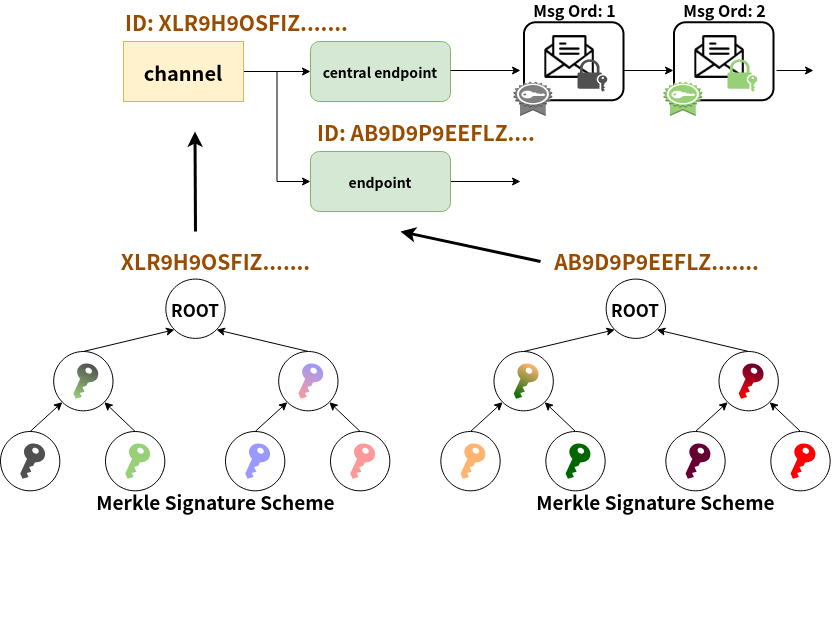
\includegraphics[width=3.5in]{mam_structure}
    \caption{With a seed, users can generate multiple channels, which can then generate multiple endpoints. The IDs of channel and endpoint are the roots of different Merkle trees in MSS. The "central endpoint" are endpoints that has ID, where $endpoint\ ID = channel\ ID$.}
    \label{fig:mam_structure}
\end{figure}

\subsection{Enable Access Control and Authentication}
\label{section:mam_features}
The access control can be enabled via encryption with NTRU\cite{NTRU}, a quantum secure cryptosystem, or Pre-shared key (PSK), to prevent random users retrieving the data from channels. If the message payload is encrypted, subscribers are required for encryption keys to decode messages. The authentication in MAM includes two aspects: source and data. Source authentication ensures the message that originates from the claimed owner, and data authentication ensures the integrity of the data from the sender. These are achieved through the MSS and One-way hash functions by validating the signature added in the signature section of the MAM bundle. However, the size of Merkle Hash Trees, that is, the size of a channel/endpoint should be determined at the start. Thus, data providers need to first decide how to distribute data products into MAM channels/endpoints before uploading data.

\subsection{Delegate MAM operations to Accel}
\label{section:ta_endpoint}
MAM builds a secure and authenticated communication protocol on top of multiple cryptosystems, which low-level devices need to spend a lot of resources with, and they may not even support built-in libraries in regular operating systems. To overcome these concerns, we propose another approach that allows data providers to delegate the MAM operations to Accel, proxy servers with high computation power, which can accelerate the interactions with Tangle while ensuring the privacy of data providers. Fig.~\ref{fig:delegation} shows how data providers can adopt MAM.

\begin{figure}[!t]
    \centering
    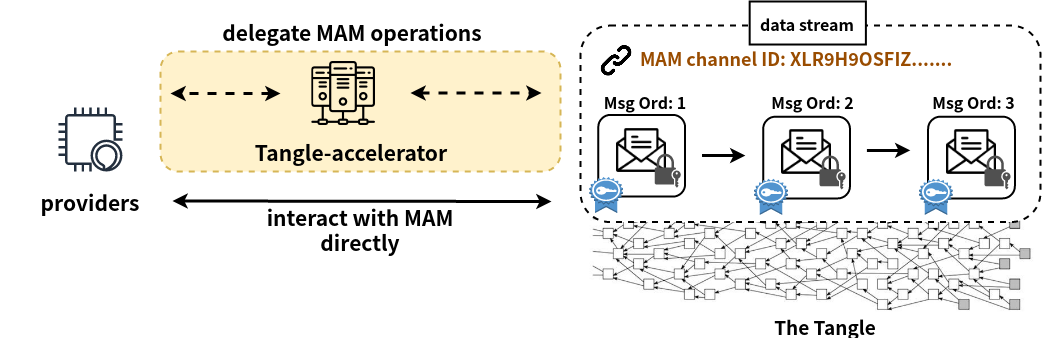
\includegraphics[width=\linewidth]{delegation}
    \caption{Data providers can use MAM in 2 ways: the provider performs MAM operations locally, and the provider delegates MAM operations to Accel.}
    \label{fig:delegation}
\end{figure}

\subsubsection{End-to-End-Encryption}
Introducing a proxy server to process all the cryptographic operations increases the risk of messages being tampered during transmission. To avoid such malicious operations, we propose another lightweight end-to-end-encryption (E2EE) upon MAM protocol. The plaintext will be encrypted with E2EE, which ensures only authorized subscribers can access the messages.

\begin{figure}[!h]
    \centering
    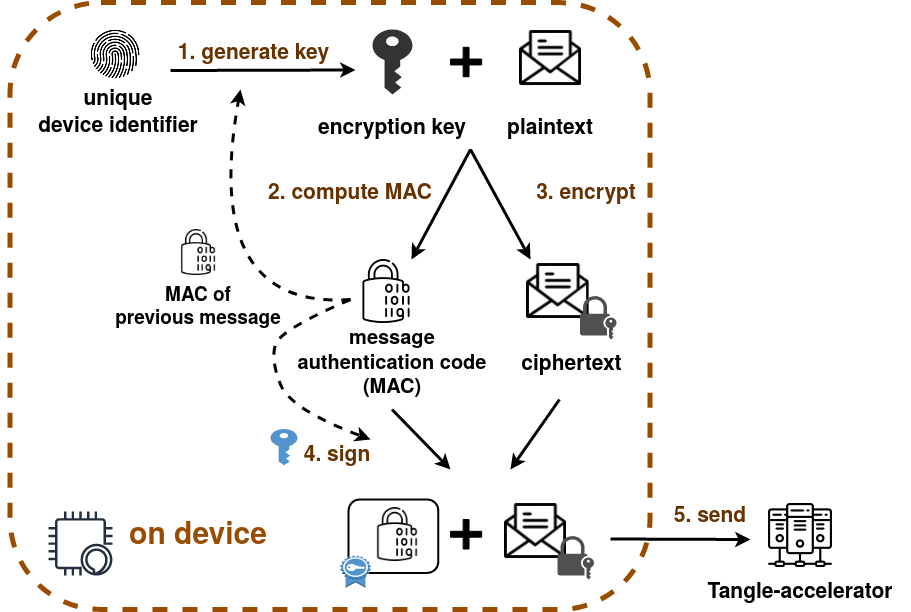
\includegraphics[width=3in]{MAM_E2EE_fold}
    \caption{The process of E2EE.}
    \label{fig:MAM_E2EE}
\end{figure}

The presented E2EE process is shown in Fig.~\ref{fig:MAM_E2EE} and illustrated below:

\begin{enumerate}
    \item Generate symmetric keys from the unique device identifier and Message Authentication Code (MAC) of the previous message with Key Derivation Function (KDF). For the first message, the sharing secret initialization information is taken as the MAC of the previous message.\label{item:1}
    \item Compute the MAC of the current message with the Hash-based Message Authentication Code (HMAC) using the symmetric key from \ref{item:1}.
    \item Apply the generated symmetric key to encrypt the message.\label{item:3}
    \item Concatenate the MACs of the current and the previous message, then sign it.\label{item:4}
    \item Send the results of \ref{item:3} and \ref{item:4}.
\end{enumerate}

The E2EE protocol combines a series of different cryptographic procedures, which can be swapped by developers to adjust different hardwares or scenarios. The elapsed time could be dropped a step more on hardwares that supported acceleration, for example, applying AES-NI can speed up AES operations around 40\% on Intel devices\cite{AES-NI-Acceleration}, and AES accelerators are integrated on some popular microcontrollers as well\cite{stm}.

\subsubsection{Time Complexity}
In this paper, we choose SHA-256 for HMAC, AES-CBC for symmetric encryption, and ECDSA P-256 for digital signature. EDSA would take constant time, since the input is fixed length. The time complexity of HMAC with SHA-256 is $O(n)$\cite{hmac_time_complexity}, and block cipher takes constant time for a single block with time complexity $O(n)$. Therefore, the E2EE protocol takes only linear time versus arbitrary string length.

\subsubsection{Issues in End-to-End-Encryption}
E2EE dramatically reduces the execution time of encryption that lowers the barries of utilizing blockchain service for low-level devices. However, Accel can tamper the messages and even spam on the requester's MAM channel, where its root is given to Accel at start. Significantly, it is risky for an edge device to connect to an Accel operating by an unknown third-party, thus connecting to a known, trustworthy Accel would be the easiest solution to prevent such attacks.

\section{Decentralized Subscription-based Data Trading Models}
\label{section:trading_model}
In this section, we illustrate how participants can join the data subscription platform, start subscribing, cancel the subscription and a discussion of refunds is illustrated.

\subsection{Prerequisite}
All participants are required to register on TangleID to get a DID document and public/private key pair for sensitive contents exchange and authentication. An Ethereum account is also needed to interact with smart contracts and transfer Ethereum tokens.

\subsection{Launch Data Products}
To launch a data product, brokers are responsible to create a Product Contract and record the metadata of the data product for data providers. The Product Contract will not accept subscriptions until brokers certify the encryption key. To certify the encryption key, the data provider first computes its digest with the hash function and sends the digest as well as the signature to brokers. The broker verifies the signature with the public key on the provider's DID document. If it's valid, the broker will sign and upload the key to the Product Contract, otherwise, the process will be aborted. The number of key uploading times is restricted in order to avoid data provider uploading fake keys frequently. If data consumers find out the encryption key does not match the provider's signature after payment, they can request a refund. Fig.~\ref{fig:key_upload} demonstrates the key uploading process to the Product Contract via a broker. Finally, the data product is launched and data providers can start uploading data.
\begin{figure}[h]
    \centering
    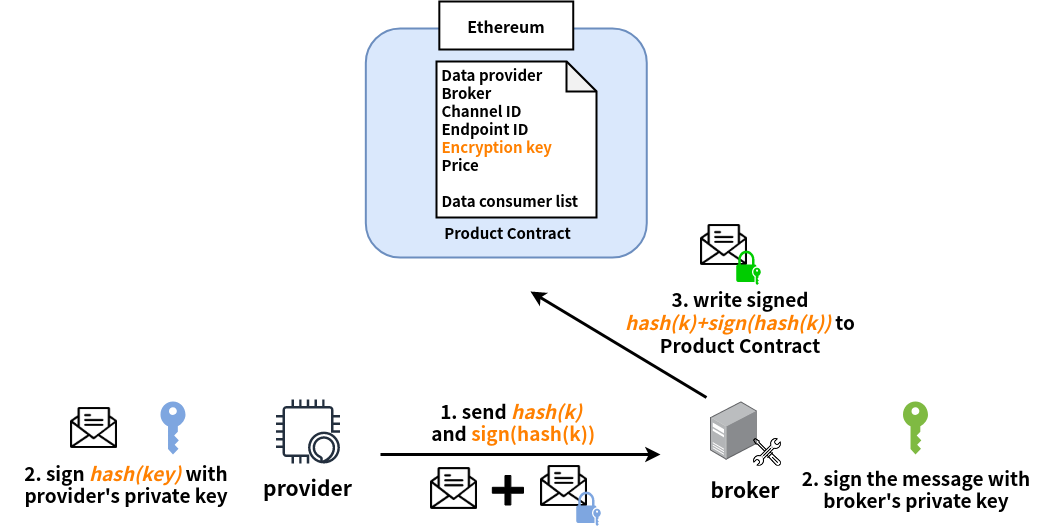
\includegraphics[width=3.5in]{key_upload}
    \caption{To add encryption key to Product Contract, the data provider sends the digest of the encryption key and the one that signed with his/her private key. After the broker receive the request, he/she signs it as well, then write the result to the Product Contract.}
    \label{fig:key_upload}
\end{figure}

\subsection{Subscribe to Data Product}
Data consumers pay subscription fees to the Product Contract of desired data products, and data providers give the encryption key of data stream instead of the files to consumers. The MAM channel/endpoint encryption key is encrypted with the public key of data consumer by the data provider and written on the Product Contract, which ensures only data consumers can decode it.

Transferring the encryption key on smart contracts instead of off-chain not only ensures the consistency of the encryption key but also prevents frauds from malicious participants, and the exchange process is transparent to the public. Furthermore, with the help of brokers and smart contracts, both data providers and consumers do not need to be online at the same time to proceed with the trading process. The key sending process is shown in Fig.~\ref{fig:key_exchange}. The subscription fee is transferred from the Product Contract to data providers when the committed data is available on MAM.

\begin{figure}[!t]
    \centering
    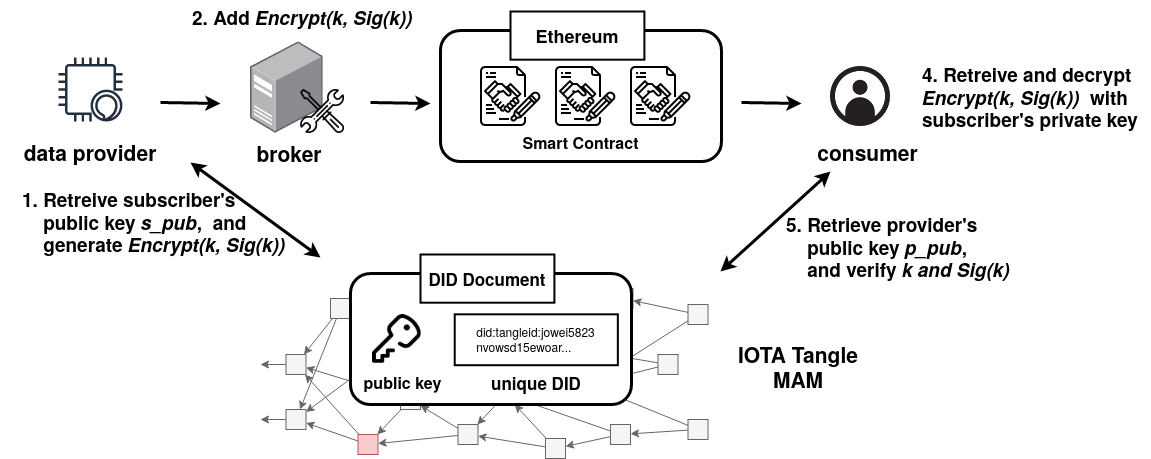
\includegraphics[width=3.5in]{key_exchange_reorganize}
    \caption{Encryption key exchange process.}
    \label{fig:key_exchange}
\end{figure}

\subsection{Unsubscribe to Data Products}
When data consumers unsubscribe to data products, they are marked as not subscribing on the Product Contract, and the withdraw function is executed to pay the fee proportionally to participants, which is defined in formula~\ref{equation:unsubscribe},~\ref{equation:unsubscribe_1},~\ref{equation:unsubscribe_2}. $i$ is the number of data when refunding condition is met, $price$  is the subscription price, $M$ is the number of expected data records, $F_{b}$ (\%) is the brokerage fee which is expressed as a percentage, $F_{t}$ is the transaction fee of the smart contract, and $F_{cancel}$ is the cancellation fee charged for unsubscription. In SaaS, the cancellation fee is a way to make sure the service providers are protected if subscribers drop out at the early stage. However, asking cancellation fee arbitrarily may cause an unfair contract that leads to the legal issue, which should be carefully studied. Finally, data provider will change the encryption key to prevent unsubscribers continue accessing the following data. The new key should be updated for the remaining subscribers.
\begin{align}
    F_{Provider}(i) &= price \frac{i-1}{M} (1-F_{b}+F_{cancel}) -F_{t} \label{equation:unsubscribe} \\
    F_{Broker}(i) &= price \frac{i-1}{M} F_{b} -F_{t} \label{equation:unsubscribe_1} \\
    F_{Consumer}(i) &= price (1-\frac{i-1}{M})(1 -F_{cancel}) -F_{t} \label{equation:unsubscribe_2}
\end{align}
\subsection{Refund}
\label{section:refund}
The refund topics are complicated in subscription services; therefore, we illustrate the challenges in this section. As subscription-based services in the real-world, participants can launch a refund in the following conditions: First, consumers launch a vote for refund when the data provider does not upload data as expected after receiving the subscription fee. It is notable that consumers can only initiate a refund after getting the data or in a certain time period. In this situation, the broker should host and set a vote timeline to count the votes, as well as handling the condition that not enough consumers join the vote. The process needs to be considered carefully. Second, brokers operate the subscription platform by earning brokerage fees, which is a deal between brokers and providers. If they cannot reach a consensus on the brokerage fee during the subscription period, brokers can launch a refund and reject to handle the product. Third, the refund could be launched by providers when they fail to maintain products as committed.

\section{Evaluations}
\label{section:evaluation}
We evaluate the cost of operating the subscription-based data trading infrastructure in two aspects: 1) the minimum cost for participants to sustain or subscribe to a data product via Product Contract. 2) the cost of adopting MAM on arbitrary devices, since it is the most commonly used component to data providers.

\subsection{Gas usage of the Product Contract}
We investigate the cost of executing a Product Contract with Ethereum web browser-based IDE Remix. On top of this evaluation, data providers can consider how to set the subscription and brokerage fee to eventually generate profits. The estimated cost is in USD, where $1\ Ether = 238\ USD$ at the time of writing, yet the price is dynamic from time to time. To conquer this condition, we analyze with a fixed range of Gas prices. According to the report of Ethereum network\cite{ethereumChart} in 2020 (January to June), we set this range from 7.3 Gwei to 26.5 Gwei, which is $7.3 \times 10^{-9}$ and $2.65 \times 10^{-8}$ Ether respectively, the minimum average and average gas price. Note that data uploading is only related to MAM operations on the Tangle without transaction fees. Therefore, the Gas estimation only includes trading processes. The high transaction fee for brokers is due to the multiple store operations in contract deployment and key certification, which takes high Gas usage according to Ethereum Yellow Paper. Therefore, it is worth exploring the usage of the non-interactive zero-knowledge protocol such as zk-SNARKS\cite{Snark} which can generate proofs off-chain and simplify the verification process. It can not only reduce network and storage cost but also improve the privacy and security of encryption keys.

\begin{table}[h]
    \caption{Transaction fees for each participant}
    \label{tab:gas}
    \centering
    \begin{tabular}{|c|c|c|c|}
        \hline
        \textbf{participant} & \textbf{Gas used} & \textbf{\makecell{minimum price \\ (USD)}} & \textbf{\makecell{maximum price \\ (USD)}} \\
        \hline
        provider & 166203 & 0.288 & 1.048 \\
        broker & 2733985 & 4.750 & 17.243 \\
        consumer & 83572 & 0.145 & 0.527  \\
        \hline
    \end{tabular}
\end{table}

\subsection{MAM Performance Evaluation}
\label{section:mam_performance}
%In the following evaluations, all devices run with the IOTA client library instead of IOTA full nodes.
MAM is the primary component to resolve the storage difficulties discussed in previous sections. The interactions between data providers and MAM can be frequent, hence it is one of the potential bottlenecks during the subscription processes. In this section, time measurement is evaluated in two MAM operations: channel/endpoint creation and message publishment. A personal computer (PC; 3.2GHz 6-core i7-8700 with 16GB DDR4 RAM) and a Raspberry Pi 3 Model B (RPi; 1.2 GHz 4-core ARM Cortex-A53 with 1GB LPDDR2 RAM) have been used to run MAM.

\subsubsection{Channel / Endpoint Creation}
The length of a channel/endpoint is $2^{height}-1$ where \textit{height} is the height of Merkle Hash Tree in MSS, and the "$-1$" is for announcing the ID of next channel or endpoint. The greater the \textit{height} of MSS, the longer the channel/endpoint, however the higher the computational power is required. In this task, both channel and endpoint creation are tested and the \textit{height} is set from 1 to 7 which is quite enough for data providers to upload data.

Fig.~\ref{fig:mam_create} shows the results of channel/endpoint creation. The time duration for each \textit{height} is the average time of running 100 rounds. Since the workflow of channel and endpoint creation are identical, the curves of the same hardware almost match. On the other hand, the elapsed time of RPi grow rapidly when \textit{height} is 5 or above. And on PC, all remain acceptable even the \textit{height} gets to 7. The results indicate that MAM channel/endpoint creation is a laborious job for data providers, and can be considered delegating to Accel.
\begin{figure*}[!htb]
\minipage{0.32\textwidth}
  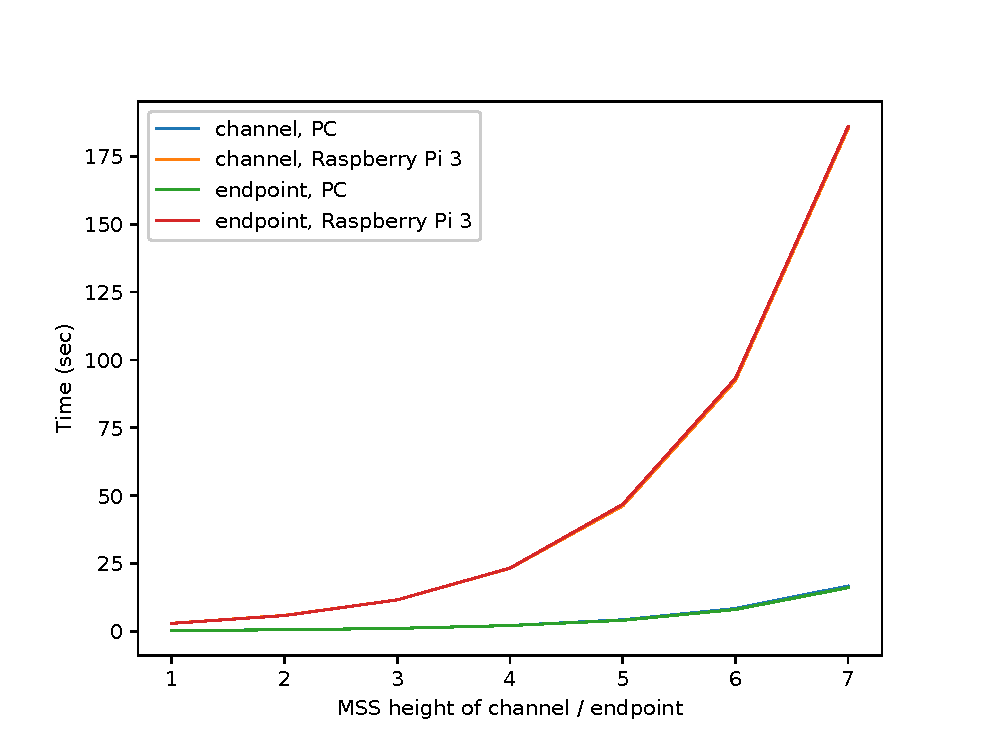
\includegraphics[width=\linewidth]{mam_create}
  \caption{Time cost of MAM creation.}\label{fig:mam_create}
\endminipage\hfill
\minipage{0.32\textwidth}
  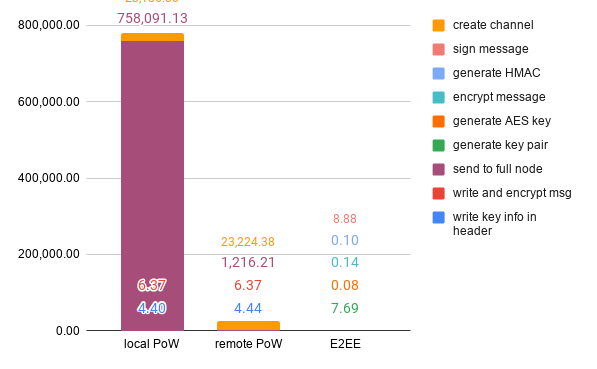
\includegraphics[width=\linewidth]{rpi3_pow}
  \caption{MAM with local PoW \newline vs. MAM with remote PoW \newline vs. Delegated MAM with E2EE}\label{fig:rpi3_pow}  
\endminipage\hfill
\minipage{0.32\textwidth}%
  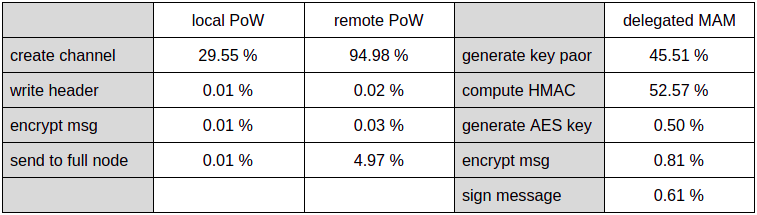
\includegraphics[width=\linewidth]{op_share}
  \caption{The percentage each operation takes in total elapsed time.}\label{fig:op_share}  
\endminipage
\end{figure*}

\subsubsection{Messages Publishment}
Publishing a message to MAM is attaching a zero-value transaction to the Tangle which requires two processes: 1.) \textbf{Tips selection}: In the IOTA protocol, a new-coming transaction needs to pick up 2 existed transactions called tips to reference and verify. The tips are provided by IOTA full nodes. 2.) \textbf{Proof-of-Work (PoW)}: An algorithm that prevents Denial of Service and spam attacks on a network.

Tips selection requires a stable network connection to wait for the response from IOTA full nodes, and PoW requires enough computation resources to perform. The time of RPi distributed widely, from 5 secs to over 2500 secs, due to the randomness of PoW. The simulation results indicate that publishing messages locally is difficult for low-level sensor devices, whereas they are the majority of hardwares in IoT scenarios. Therefore, the devices can delegate MAM operations to Accels while ensuring the profit and privacy of providers through E2EE, which can lower the threshold to participate the subscription platform. Fig.~\ref{fig:rpi3_pow} shows the time cost of sending a MAM message with 500 bytes payload with local PoW, remote PoW and E2EE on RPi. However, improving the performance of MAM is still a direction that worth working on.

\subsection{MAM vs. the delegated MAM}
\label{section:smart_contract_evaluation}
\subsubsection{Experiment}
From Fig.~\ref{fig:op_share}, send to full node (i.e., prepare and attach the message) and create a channel take most of the time to broadcast a MAM message. In Fig.~\ref{fig:rpi3_pow}, we apply remote PoW to reduce the time of the former, and we delegate MAM to Accel to improve the later. This strategy outperforms the original MAM, particularly for different payload sizes. To better understand the time cost of MAM and delegated MAM, the measurement only contains the MAM operations running on device, where PoW and internet transmission are not included. Furthermore, the MAM channel creation and E2EE asymmetric key pair generation are not included either, since the two operations are rarely executed. In E2EE, we respectively choose SHA-256 for HMAC, AES-CBC for symmetric encryption, and Curve P-256 for ECDSA.

The measurement for original MAM includes: 1.) write the key information to the header, 2.) encrypt and write the message, 3.) publish final message to the Tangle. And the measurement for delegated MAM (E2EE) includes: 1.) generate a symmetric key for encryption, 2.) Hash the message, 3.) encrypt the message, 4.) send the message to Accel. The result is shown in Table.~\ref{tab:mam_vs_e2ee}.

\begin{table}[htbp]
    \caption{Compare the performance between MAM and E2EE on RPi}
    \label{tab:mam_vs_e2ee}
    \centering
        \begin{tabular}{|c||c|c|}
        \hline
            \textbf{size (bytes)} & \textbf{MAM(ms)} & \textbf{E2EE(ms)} \\
            \hline
            100 & 20.28 & 9.21 \\
            500 &  26.92 & 9.27 \\
            900 & 32.02 &  9.35  \\
            1300 & 36.67 & 9.41 \\
            1700 & 40.55 & 9.54 \\
            \hline
        \end{tabular}
\end{table}

The result shows that the elapsed time of E2EE is obviously less than MAM, and E2EE results in a slowly increasing time for different data sizes. This shows that E2EE enables resource-constrained hardwares to join the data subscription economy as providers and ensures tamperless data transmission to Accel.

\section{Conclusion and Future Work}
\label{section:conclusion}
This paper aims to propose a highly decentralized, autonomous publish/subscribe model that combines data storage and trading together in order to ensure the digital rights of both data providers and consumers during the dynamic data streaming trading. To clarify the data ownership and identity verification, the data stream is stored on the Tangle, transmitted through MAM, and automated by Ethereum smart contracts in our design. Compared to previous works, we (1) identify a trustless data trading infrastructure, (2) ensure the confidentiality of scalable IoT-based sensor data, and (3) consolidate the economic incentives in the entire ecosystem. Meanwhile, we consider the heavy workload of the low-level sensors, conduct an experiment which authenticates the data providers to delegate the MAM operations to TAs, and conclude that the performance of the E2EE approach is more fitting than the MAM solution. In particular, this work discusses the refund mechanism for subscription-based IoT data trading: Launching, voting, and implementing the refunding procedure.

Our work has a main focus on the subscription-based model and relative experiments. And the next step is extending it to:
\begin{enumerate}
    \item reduce the use of Gas in key-agreement protocol and consider the possibility of the zero-knowledge proof to lower transaction costs;
    \item analyze the minimum number of brokers needed for the system and the procedures of the refund mechanism;
    \item develop a product portal for consumers to find their interested tagging or data products as well as a ranking system to maintain the quality, without violating the privacy.
\end{enumerate}

Finally, a decentralized model enables the data stream trading by shifting risks, and correspondingly, the digital rights of its participants deserve a guarantee, which is provided with the automated system.

\bibliographystyle{IEEEtran}
\bibliography{references}

\end{document}